\documentclass{article}
\usepackage{graphicx}
\usepackage{lmodern}  % for bold teletype font
\usepackage{amsmath}  % for \hookrightarrow
\usepackage{xcolor}   % for \textcolor
\usepackage{listings}
\lstset{
  basicstyle=\ttfamily,
  columns=fullflexible,
  frame=single,
  breaklines=true,
  postbreak=\mbox{\textcolor{red}{$\hookrightarrow$}\space},
}
%Enumering lower case roman numerals
%\renewcommand{\theenumi}{\roman{enumi}}   
%\renewcommand{\labelenumi}{\theenumi)}


\begin{document}

\title{\vspace{-2.0cm}Drone Programming Introduction\\IDP 2022}

\author{Neil Dhami \\EE18BTECH11031	}

\maketitle
%-------------------------------------------------------------------------------
Download all python codes from 
\begin{lstlisting}
https://github.com/neildhami18/IITH_Academics/DroneIDP-2022/Manual-2/codes
\end{lstlisting}

%
and latex-tikz codes from 
%
\begin{lstlisting}
https://github.com/neildhami18/IITH_Academics/DroneIDP-2022/Manual-2/
\end{lstlisting}

\section{Introduction}
This manual is a guide on how to connect and configure a Raspberry Pi (RPi) so that it is able to communicate with a flight controller using the MAVLink protocol over a serial connection. DroneKit-Python allows you to control your flight controller using the Python programming language. 

\section{UAV setup}
Make sure that the UAV is fully calibrated ready to fly in the manual/stabilize mode. In case the GPS was not connected, connect it to the flight controller and re-calibrate the compass. Reboot the flight controller and carry the UAV to an open ground. On connecting the flight controller with GCS (Mission Planner), a GPS lock should be obtained. 

\section{Raspberry Pi Setup}
Flash a SD card with latest Raspberry Pi imager. While installation, it is recommended to select mobile hot-spot as SSID. Post installation, power up the raspberry pi, turn on mobile hot-spot, open termux and connect to the raspberry pi via the following commands. Make sure only one device (Raspberry Pi) is connected to the hot-spot.

\subsection{Establishing a connection}
Type the following commands for establishing the connection to RPi.
\begin{itemize}
    \item Know the IP address of your device (mobile):
    \begin{lstlisting}[language=bash]
    $ ifconfig
    \end{lstlisting}
    \item Search for IP address of RPi
    \begin{lstlisting}[language=bash]
    $ nmap 192.168.abc.1/24
    \end{lstlisting}
    \item Connect to RPi terminal
    \begin{lstlisting}[language=bash]
    $ ssh pi@192.168.abc.xyz
    \end{lstlisting}
    
        
\end{itemize}

Figures for reference:
\begin{figure}[!htb]
            \minipage{0.32\textwidth}
              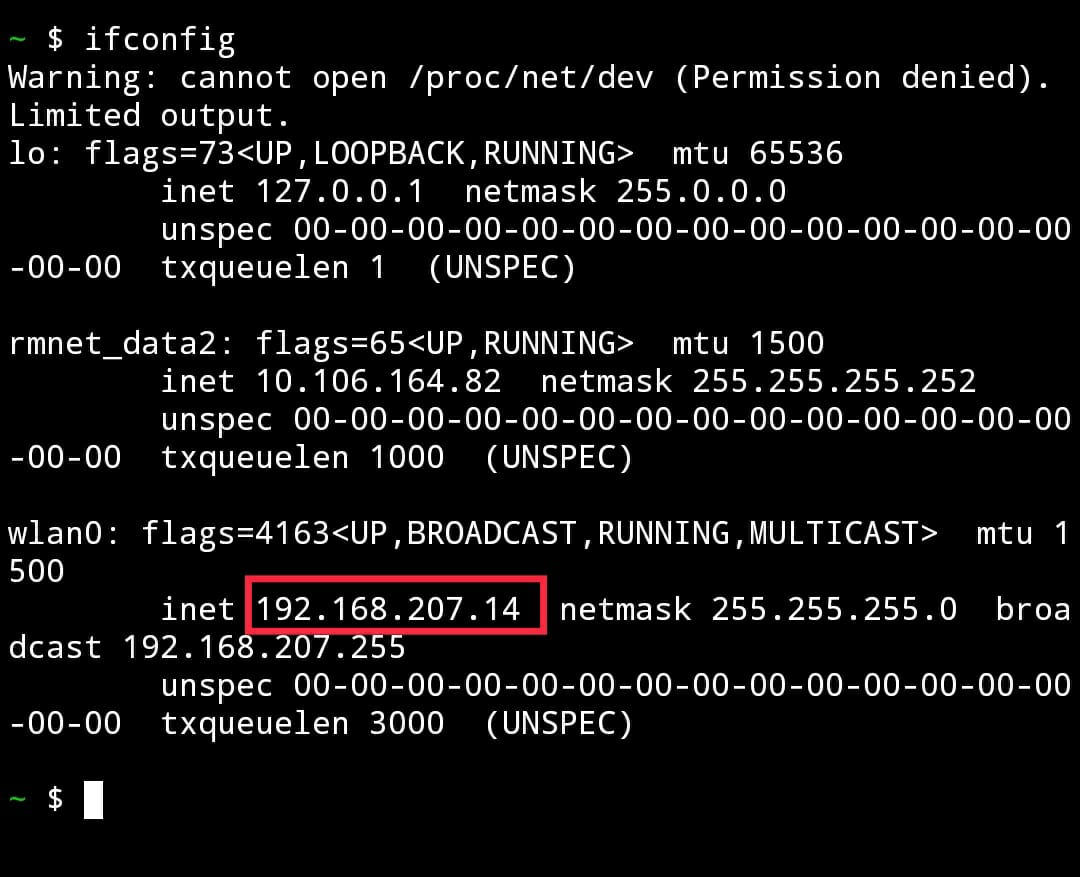
\includegraphics[width=\linewidth]{./figs/termux/ifconfig.jpeg}
              \caption{Mobile IP Address}\label{fig:awesome_image1}
            \endminipage\hfill
            \minipage{0.32\textwidth}
              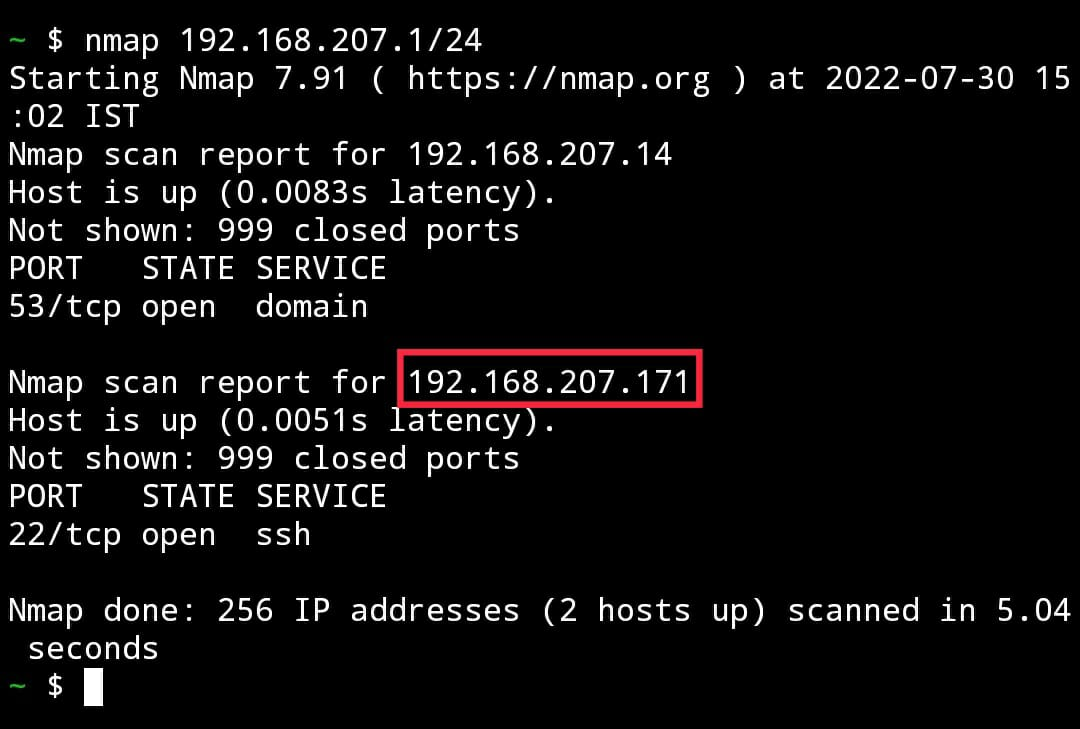
\includegraphics[width=\linewidth]{./figs/termux/nmap.jpeg}
              \caption{RPi IP Address}\label{fig:awesome_image2}
            \endminipage\hfill
            \minipage{0.32\textwidth}%
              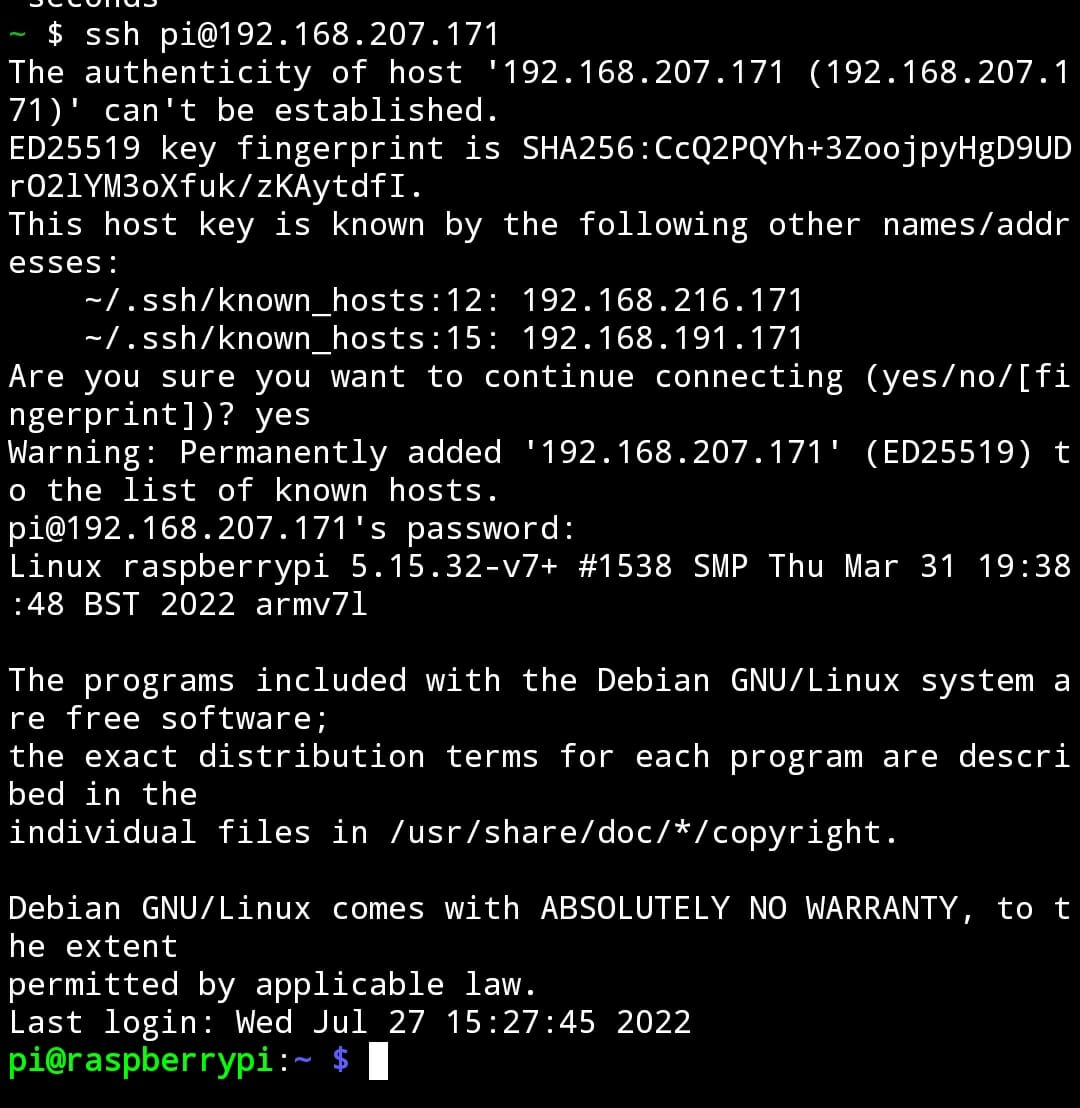
\includegraphics[width=\linewidth]{./figs/termux/ssh.jpeg}
              \caption{Connect to RPi}\label{fig:awesome_image3}
            \endminipage
\end{figure}

\subsection{Installing packages}
Install the following packages
\begin{lstlisting}[language=bash]
    $ sudo apt-get update
    $ sudo apt-get upgrade
    $ sudo apt-get install python3-pip
    $ sudo apt-get install python3-dev
    $ sudo apt-get install screen python3-wxgtk4.0 python3-lxml
    $ pip install future pyserial dronekit
    $ pip install mavproxy
\end{lstlisting}
 
\noindent Setup RPi for UART communication
\begin{lstlisting}[language=bash]
    $ sudo raspi-config
\end{lstlisting}
Select the Serial Port option in Interface Options.\\
Disable the serial login shell and enable the serial port hardware interface. 
\\
\\
Now, connect a the RPi (USB) to the flight controller (micro-USB) via a USB cable. \\
\\
\textbf{Note:} RPi can be powered through the GPIO pins. Connect 5V and GND pins of the flight controller to the corresponding GPIO pins of RPi. Now the battery shall power the flight controller, which in-turn would power the RPi through GPIO and take commands from RPi through the USB. \\

\textbf{Additional:} For better space utilisation, the flight controller could be mounted over the RPi through standoff screws and a plate as shown below:
\begin{figure}[!htb]
            \minipage{0.6\textwidth}
              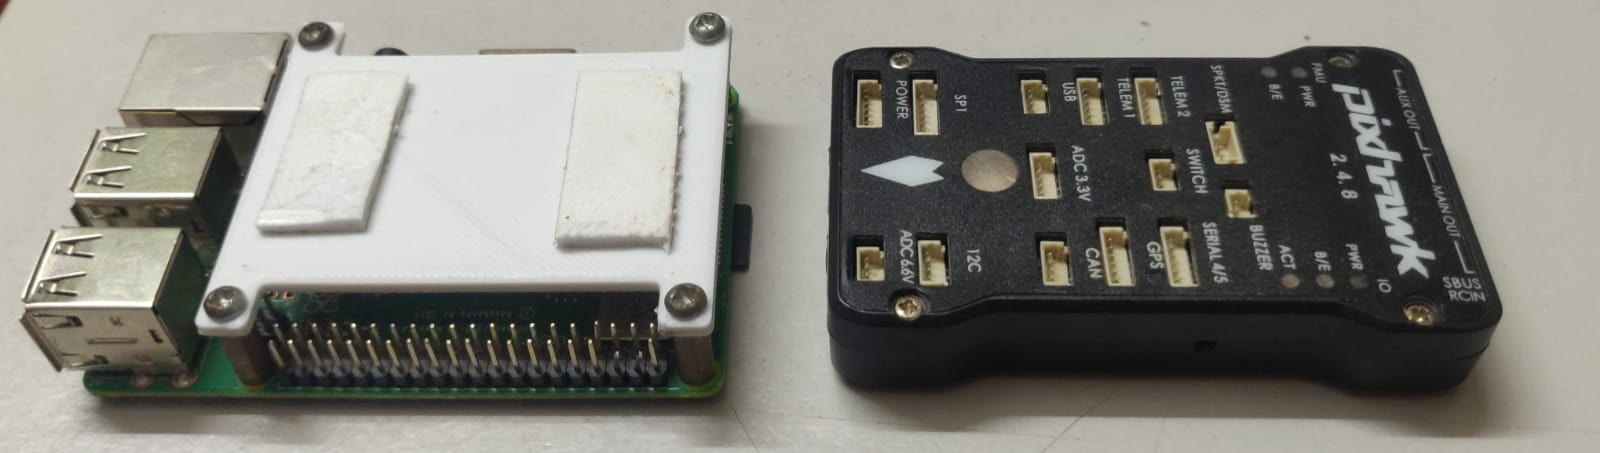
\includegraphics[width=\linewidth]{./figs/hardware/separate.jpeg}
            \endminipage\hfill
            \minipage{0.3\textwidth}
              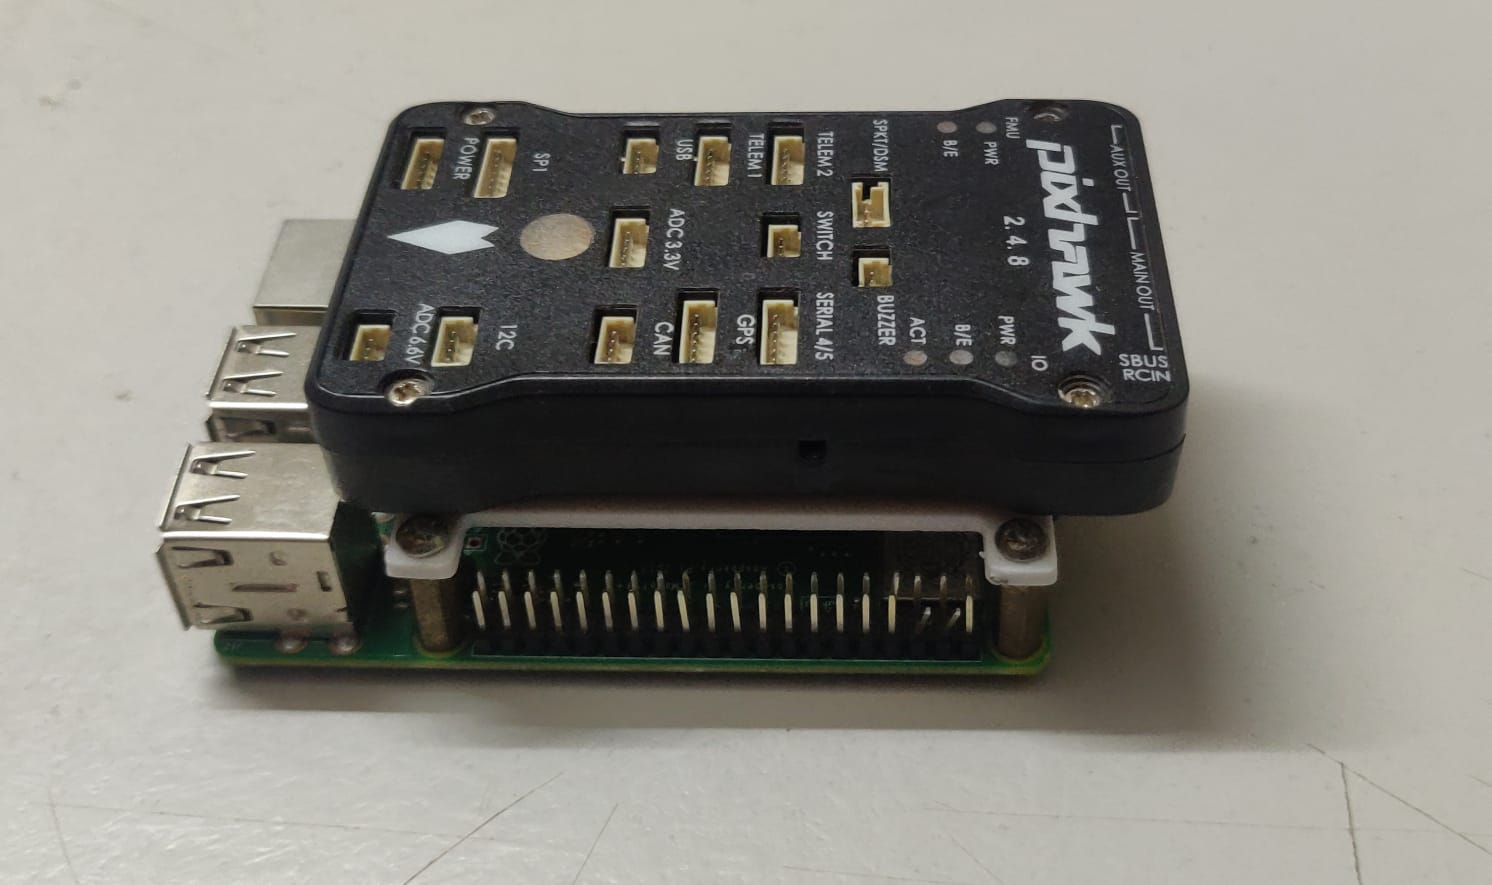
\includegraphics[width=\linewidth]{./figs/hardware/together.jpeg}
            \endminipage\hfill
\end{figure}
The STL file for the plate:
\begin{lstlisting}
https://github.com/neildhami18/IITH_Academics/DroneIDP-2022/Manual-2/hardware
\end{lstlisting}


Type the following command and enter:
\begin{lstlisting}[language=bash]
    $ mavproxy.py --master=/dev/ttyACM0 
\end{lstlisting}
The terminal should display information including arducopter version, flight mode etc. Change the mode to GUIDED by using the following command:
\begin{lstlisting}[language=bash]
    mode GUIDED
\end{lstlisting}
Connect the battery and power up the UAV. Make sure propellers are removed. Turn on your RC Transmitter. Type the command:
\begin{lstlisting}[language=bash]
    arm throttle
\end{lstlisting}
The motors should start rotating.

\section{Exercises}
\subsection{Problem-1}
Write a basic dronekit mission in python to arm the UAV.

\begin{lstlisting}[language=Python]
from dronekit import connect, VehicleMode, LocationGlobalRelative
import time
import socket
import math
import argparse

def connectMyCopter():
    parser = argparse.ArgumentParser(description='commands')
    parser.add_argument('--connect')
    args = parser.parse_args()
    connection_string = args.connect
    vehicle = connect(connection_string, wait_ready=True)
    return vehicle

def arm():
    '''    
    while vehicle.is_armable==False:
        print("Waiting for vehicle to become armable")
        time.sleep(1)
    print("Vehicle is now armable")
    '''
    vehicle.armed=True
    while vehicle.armed==False:
        print("Waiting for drone to be armed..")
        time.sleep(1)
    print("Vehicle is now armed..")
    print("Props are spinning... LOOKOUT!!..")
    return None

# Main
vehicle = connectMyCopter()
arm()
print("End of script..")

\end{lstlisting}

Run the program through the following command:
\begin{lstlisting}[language=bash]
    $ python arming.py --connect=/dev/ttyACM0
\end{lstlisting}

\subsection{Problem-2}
Write a dronekit mission in python to fly the drone to a particular input altitude and then land.\\
The takeoff function could be defined as:
\begin{lstlisting}[language=Python]
def arm_and_takeoff(Altitude):
    '''
    while not vehicle.is_armable:
        print("Waiting for vehicle to become armable")
        time.sleep(1)
    '''
    vehicle.mode = VehicleMode("GUIDED")
    while vehicle.mode!="GUIDED":
        print("Waiting for vehicle to enter GUIDED mode")
        time.sleep(1)

    vehicle.armed=True
    while vehicle.armed==False:
        print("Waiting for vehicle to become armed.")
        time.sleep(1)

    vehicle.simple_takeoff(Altitude)
    
    while True:
        print("Current Altitude: %d"%vehicle.location.global_relative_frame.alt)
        if vehicle.location.global_relative_frame.alt>=Altitude*.90:
            break
        time.sleep(1)

    print("Altitude Reached!!!")
    return None

\end{lstlisting}

\subsection{Problem-3}
Write a dronekit mission in python to fly the drone to a particular altitude, traverse in various directions with a particular velocity and land.\\
The velocity function could be defined as:
\begin{lstlisting}[language=Python]
def set_velocity(Vx,Vy,Vz):
    msg = vehicle.message_factory.set_position_target_local_ned_encode(
            0,
            0,0,
            mavutil.mavlink.MAV_FRAME_BODY_OFFSET_NED,
            0b0000111111000111, #BITMASK -> Consider only the velocities
            0,0,0, #Position
            Vx,Vy,Vz, #Velocity
            0,0,0, #Accelerations
            0,0)
    vehicle.send_mavlink(msg)
    vehicle.flush()

\end{lstlisting}

\section{Notes}
\begin{itemize}
    \item Ensure that a long thread is tied to the UAV while experimenting with dronekit missions.
    \item If the UAV seems to be not following the path or mission, one can control it using the RC transmitter. 
    \item Always perform the experiments in a large open ground. 
    \item Ensure that the LiPo battery is charged with a Voltage grater than 11.5V.
\end{itemize}

\end{document}

